\section{Introduction}



\section{A distribution that is hard for standard graph neural networks.}





\section{Preliminaries}

\section{Graph Theoretical Foundations}

In this section, we establish the fundamental definitions that will be used throughout this paper.

\subsection{Undirected Graph}
An \textit{undirected graph} is defined as a pair $G = (V, E)$, where:
\begin{itemize}
    \item $V$ is a finite set of vertices (or nodes).
    \item $E \subseteq \{ \{u,v\} \mid u,v \in V, u \neq v\}$ is a set of edges, where each edge is an unordered pair of distinct vertices.
\end{itemize}
Since the graph is undirected, if $\{u,v\} \in E$, then there exists a connection between $u$ and $v$, and the relationship is bidirectional.

A useful way to represent $G$ is through its \emph{adjacency matrix} $\mathbf{A} \in \{0,1\}^{n \times n}$, where $n = |V|$ is the number of nodes. The adjacency matrix is defined as:

\begin{equation}
A_{ij} =
\begin{cases}
    1, & \text{if } \{i,j\} \in E, \\
    0, & \text{otherwise}.
\end{cases}
\end{equation}

Since the graph is undirected, $\mathbf{A}$ is symmetric, meaning that $A_{ij} = A_{ji}$ for all $i,j \in V$. The diagonal entries $A_{ii}$ are typically zero unless self-loops are explicitly included in the graph. This matrix representation provides a convenient way to encode the graph structure for computational methods, including graph neural networks.

\subsection{Clique}

A \textit{clique} in a graph $G = (V, E)$ is a subset of vertices $C \subseteq V$ such that every pair of vertices in $C$ is adjacent, meaning that for all $u, v \in C$ with $u \neq v$, the edge $\{u,v\}$ is present in $E$. 

A \textit{clique} in a graph $G = (V, E)$ is a subset of vertices $C \subseteq V$ such that every pair of vertices in $C$ is adjacent, meaning that for all $u, v \in C$ with $u \neq v$, the edge $\{u,v\}$ is present in $E$. 

The \textit{k-clique problem}, which asks whether a graph contains a clique of size $k$, is NP-complete when $k$ is part of the input \citep{karp1972reducibility}, but for a fixed constant $k$, it can be solved in polynomial time by enumerating all $\binom{|V|}{k}$ possible subsets of vertices and checking for completeness. More specifically, \citet{vassilevska2009efficient} show that the problem can be solved in $O\left(\frac{n^k}{(\varepsilon \log n)^{k-1}}\right)$ time and $O(n^\varepsilon)$ space for all $\varepsilon > 0$, achieving an improvement over the naive $O(n^k)$ approach.


\subsection{Graph Coloring}
A \textit{proper coloring} of a graph $G = (V, E)$ is an assignment of colors to vertices such that no two adjacent vertices share the same color. Formally, a function $f: V \to \{1,2,\dots,r\}$ is an $r$-coloring if for every edge $\{u,v\} \in E$, it holds that $f(u) \neq f(v)$. The \textit{chromatic number} $\chi(G)$ is the smallest integer $r$ for which an $r$-coloring exists.

The problem of determining whether a graph can be colored with at most $r$ colors, known as the \textit{graph coloring problem}, is NP-complete for general graphs when $r \geq 3$ \citep{karp1972reducibility}. However, for fixed values of $r$, specialized algorithms can solve the problem more efficiently. In particular, the $3$-coloring problem can be solved in $O(1.3289^n)$ time using an improved branching algorithm \citep{beigel2000finding}. 

\subsection{\textit{k}-Clique vs \textit{r}-Coloring Problem}




The \textit{$k$-clique vs. $r$-coloring problem} is a classification problem. Given integers $k$ and $r$, with $r < k$, and a graph $G$ that is promised to either contain a $k$-clique or be $r$-colorable, the task is to determine which is the case. While both the $k$-clique and $r$-colorability problems are individually NP-complete, this specific problem is not classified as NP-complete since the input graph satisfies exactly one of the two mutually exclusive properties.

This problem can be solved efficiently in certain graph classes, such as perfect graphs and their generalizations. In perfect graphs, the chromatic number equals the size of the largest clique, simplifying the determination of $r$-colorability and the presence of $k$-cliques. \todo{elaborate on why this helps, and why k and r can be calculated in polynomial time} For general graphs, an efficient approach relies on the Lovász theta function, $\vartheta(G)$. The Lovász Sandwich Theorem establishes the bounds:
\begin{equation}
    \alpha(G) \leq \vartheta(G) \leq \bar{\chi}(G),
\end{equation}
\citep{lovasztheta}
where $\alpha(G)$ is the independence number, representing the size of the largest independent set in $G$, and $\bar{\chi}(G)$ is the fractional chromatic number, a relaxation of the chromatic number that allows fractional color assignments. While computing $\alpha(G)$ and $\bar{\chi}(G)$ is NP-hard, the Lovász theta function is efficiently computable via semidefinite programming (SDP), making it an efficient way of separating the two classes. 


% \begin{enumerate}
%     \item The graph $G$ contains a clique of size at least $k$, i.e., there exists a subset $C \subseteq V$ with $|C| \geq k$ such that every pair of vertices in $C$ is connected.
%     \item The graph $G$ can be colored using at most $r$ colors, i.e., there exists a valid $r$-coloring function $f: V \to \{1,2,\dots,r\}$.
% \end{enumerate}

% This problem is significant in theoretical computer science and combinatorial optimization, as it relates to NP-hard problems such as \textsc{Clique} and \textsc{Graph Coloring}. The interplay between maximum clique size and chromatic number has implications in graph theory, information theory, and constraint satisfaction problems.



\subsection{Graph Convolutional Networks}
\label{sec:GCN}

To distinguish r-colorable graphs from graphs with k-cliques, we adopt the
\textbf{Graph Convolutional Network (GCN)} model proposed by \citet{GCNKipf2016} as the
core model in our pipeline.

\paragraph{Local Graph Convolutions.}  
Each node $i$ in the graph is represented with an \emph{embedding}, a vector in $\mathbb{R}^{d_{\ell}}$, where $ d_{\ell} $ is the dimensionality of the embedding at layer $ \ell $, commonly described as the number of channels. Initially ($\ell = 0$), this embedding is simply the node’s feature vector. These features can be combined into the matrix $\mathbf{H}^{(\ell)} \in \mathbb{R}^{n \times d_{\ell}}$, where each row corresponds to the embedding of a node.  

A \emph{Graph Convolutional Network (GCN) layer} updates node embeddings by aggregating information from neighboring nodes through applying a learned transformation. This transformation is parameterized by a trainable weight matrix $ \mathbf{W}^{(\ell)} \in \mathbb{R}^{d_{\ell} \times d_{\ell + 1}} $, which maps embeddings from dimension $ d_{\ell} $ to a new dimension $ d_{\ell+1} $ at the next layer. The node embeddings are updated as follows:

\begin{equation}   
    \mathbf{H}^{(\ell+1)} 
    = \sigma\!\Big(
        \widetilde{\mathbf{D}}^{-\frac12} \,
        \widetilde{\mathbf{A}} \,
        \widetilde{\mathbf{D}}^{-\frac12} \,
        \mathbf{H}^{(\ell)} \,
        \mathbf{W}^{(\ell)}
    \Big),
\end{equation}

where $ \tilde{\mathbf{A}} = \mathbf{A} + \mathbf{I} $ is the adjacency matrix with added self-loops to ensure that each node retains information from its own embedding. $ \tilde{\mathbf{D}}_{ii} = \sum_j \tilde{\mathbf{A}}_{ij} $ is a diagonal degree matrix that normalizes the adjacency matrix. Lastly, $ \sigma(\cdot) $ is a nonlinear activation function such as ReLU or sigmoid, which is crucial for enabling the model to learn complex, non-linear relationships—without it, the layer would merely perform a linear transformation, limiting the network’s expressive power.  

Stacking multiple GCN layers allows each node embedding to incorporate information from progressively larger neighborhoods. This is because each layer aggregates features from a node’s immediate neighbors. With each additional layer, a node’s representation is updated based on its direct neighbors, which themselves have already integrated information from their own neighbors in the previous layer. Consequently, deeper GCNs enable nodes to capture higher-order structural and semantic information across the graph.

% \paragraph{Local Graph Convolutions.}
% Each node $i$ in the graph is represented with an \emph{embedding}, a vector in $\mathbb{R}^{d_{\ell}}$. Initially, this embedding is simply the node features. These features can be combined into the matrix $\mathbf{H}^{(\ell)} \in \mathbb{R}^{n \times d_{\ell}}$, where each row corresponds to the embedding of a node.

% A \emph{Graph Convolutional Network (GCN) layer} is a transformation that updates node embeddings, by aggregating information from neighboring nodes. A GCN layer is defined by its trainable weight matrix $\mathbf{W} \in \mathbb{R}^{d_\ell \times d_{\ell + 1} }$. The node embeddings in a graph are then updated as follows:

% \begin{equation}   
%     \mathbf{H}^{(\ell+1)} 
%     = \sigma\!\Big(
%         \widetilde{\mathbf{D}}^{-\frac12} \,
%         \widetilde{\mathbf{A}} \,
%         \widetilde{\mathbf{D}}^{-\frac12} \,
%         \mathbf{H}^{(\ell)} \,
%         \mathbf{W}^{(\ell)}
%     \Big),
% \
% \end{equation}

% where $\tilde{A} = A + \mathbb{I}$ is the adjacency matrix $A$ of the node, with the identity matrix representing self-loops added to ensure the node's own embeddings are preserved. $\tilde{D}_{ii} = \Sigma_j \tilde{A}_{ij}$ is a diagonal matrix representing the degree of node $i$. Lastly, $\sigma(\cdot)$ is a nonlinear function such as the sigmoid or ReLU function, without which, the layer would just be a linear transformation unable to represent non-linear and thus arbitrary functions.  Stacking multiple GCN layers allows each node embedding to incorporate information from progressively larger neighborhoods. This is because each layer aggregates features from a node’s immediate neighbors. With each additional layer, a node’s representation is updated based on its direct neighbors, which themselves have already integrated information from their own neighbors in the previous layer. 

\paragraph{Graph-Level Classification.}
While GCNs were originally popularized for node-level classification tasks, our objective is
to classify entire graphs according to whether it is $r$-colorable or contains an $k$-clique. To adapt the GCN to graph-level classification, we apply global averaging across all nodes after the final GCN layer.
\begin{equation}
   \mathbf{z} 
   = \mathrm{mean}\bigl(\mathbf{H}^{(L)}\bigr) \quad \in \mathbb{R}^{d_L}
\end{equation}
where $\mathbf{H}^{(L)} \in \mathbb{R}^{N \times d_{L}}$ is the final layer output, and
$\mathrm{mean}(\cdot)$ aggregates node embeddings into a single graph-level representation $\mathbf{z}$. We then feed $\mathbf{z}$ into one or more fully connected layer(s), ending in a single output neuron used for classification. We detail the full architecture and hyperparameters in \cref{sec:experiments}.
\todo{Fix reference when this section is written}

\paragraph{Tok-k pooling}

In graph neural networks, pooling methods help reduce the size of a graph while preserving critical structural and feature-based information, making them particularly useful for tasks that depend on specific substructures. Top-K Pooling, as developed and discussed by \citet{topk1,topk2,topk3}, selectively retains the most informative nodes based on learnable importance scores. This allows the model to focus on regions of the graph that are most relevant to a given classification task. When determining whether a graph is $r$-colorable or contains a $k$-clique, certain nodes and their connections are far more influential than others. By using Top-K Pooling, the model can prioritize these key regions, reducing irrelevant complexity while retaining the features necessary to distinguish between different graph classes. The top-k algorithm is shown in \cref{alg:topk}, where $\odot$ is elementwise multiplication.

\begin{algorithm}
\caption{Top-K Pooling Algorithm}
\label{alg:topk}
\begin{algorithmic}[1]
    \State \textbf{Input:} Node feature matrix $\mathbf{X} \in \mathbb{R}^{N \times d}$, adjacency matrix $\mathbf{A} \in \mathbb{R}^{N \times N}$, learnable projection vector $\mathbf{p} \in \mathbb{R}^{d}$, pooling ratio $k$
    \State \textbf{Output:} Pooled node features $\mathbf{X'}$, pooled adjacency matrix $\mathbf{A'}$
    \vspace{0.2cm}
    
    \State \textbf{Compute node importance scores:}
    \[
    \mathbf{y} = \frac{\mathbf{X} \mathbf{p}}{\|\mathbf{p}\|}
    \]
    
    \State \textbf{Select top-k nodes based on scores:}
    \[
    \mathbf{i} = \text{top-k}(\mathbf{y}, k)
    \]
    
    \State \textbf{Update node features:}
    \[
    \mathbf{X'} = (\mathbf{X} \odot \tanh(\mathbf{y}))_{\mathbf{i}}
    \]
    
    \State \textbf{Update adjacency matrix:}
    \[
    \mathbf{A'} = \mathbf{A}_{\mathbf{i}, \mathbf{i}}
    \]

    \State \textbf{Return} $\mathbf{X'}$, $\mathbf{A'}$
\end{algorithmic}
\end{algorithm}

% Formally, top-k takes a graph defined by the feature-matrix $\mathbf{X}$ and the adjacency matrix $\mathbf{A}$, and calculates the pooled versions $\mathbf{X'}$ and $\mathbf{A'}$ as shown in 

\paragraph{Model rationale}
\todo{Rewrite and reposition}
We posit that a Graph Convolutional Network (GCN) is particularly suitable for separating r-colorable graphs from k-clique graphs due to its ability to effectively process both node features and the structural relationships defined by adjacency. GCNs should be able to capture the high-degree patterns of cliques and distinguish these from r-colorable configurations by aggregating degree information in the context of each node’s neighbors. They also excel at handling irregular graph structures, making them versatile for graphs of varying sizes.

% \paragraph{Model rationale}
% From a purely combinatorial perspective, detecting large cliques or verifying whether a graph is r-colorable presents significant challenges (see Section~\ref{sec:cliques_coloring}). Our hypothesis posits that Graph Convolutional Networks (GCNs) naturally leverage local structures—dense subgraph patterns indicative of cliques and neighborhood sparsity. By propagating features through the graph, GCNs effectively integrate multi-hop connectivity, which may correlate with specific structural patterns. Consequently, when trained on examples that are either r-colorable or contain k-cliques (or labeled with a more detailed classification scheme), the network can learn representations that distinguish between these two cases.


\section{Graph generation}

% In this section we describe how we generate random graphs that either belong to the r-colorable group or the k-clique group. For the r-colorable graphs, the nodes are first randomly given a color, and then edges are randomly assigned with probability \deprob for each pair of nodes with different colors. For the k-clique graphs, $k$ nodes are first chosen to be part of a clique, and fully connected before edges are added randomly with \deprob for all possible pairs of nodes. Each node in a GNN is associated with one or more features. For our experiments, we use the degree of the node as its feature. \Cref{alg:r-colorable,alg:k-clique} describe the graph generation algorithms in more detail.

In this section, we outline the process for generating random graphs belonging to either the $r$-colorable group or the $k$-clique group. For $r$-colorable graphs, each node is randomly assigned a color, and edges are added between nodes of different colors with a probability of $p$. For $k$-clique graphs, $k$ nodes are first selected to form a fully connected clique, after which additional edges are randomly added between all node pairs with probability $q$. In a GNN, each node is associated with one or more features; in our experiments, we use node degree as the sole feature. \Cref{alg:r-colorable,alg:k-clique} provide a detailed description of the graph generation algorithms.


\begin{algorithm}
\caption{Generating a Graph with an $k$-Clique}
\label{alg:k-clique}
\begin{algorithmic}[1]
    \Require 
        \begin{itemize}
            \item $N$: Total number of nodes in the graph
            \item $k$: Size of the clique
            \item $p$: Probability of adding edges outside the clique.
        \end{itemize}
    \Ensure A graph with a fully connected $k$-clique and additional edges based on $p$.

    \State \textbf{Select Nodes for the Clique:}
        \begin{itemize}
            \item Randomly choose $k$ nodes from the total $N$ to form the clique.
        \end{itemize}
    
    \State \textbf{Create Clique Edges:}
        \begin{itemize}
            \item For every pair of nodes in the clique, add an edge between them.
        \end{itemize}

    \State \textbf{Create Edges for Other Nodes:}
        \begin{itemize}
            \item For all pairs of nodes that are not both in the clique:
            \begin{itemize}
                \item Add an edge with probability $p$ between those nodes.
            \end{itemize}
        \end{itemize}

    \State \textbf{Combine Edges:}
        \begin{itemize}
            \item Merge the edges from the clique with the edges between other nodes.
        \end{itemize}

    \State \textbf{Generate Node Features:}
        \begin{itemize}
            \item For each node, compute its degree. Use this as the node's feature.
        \end{itemize}

   \State \textbf{Output: Adjacency Matrix, Node Features}
        \begin{itemize}
            \item Construct an adjacency matrix $\mathbf{A}$ from the list of edges.
            \item Create a feature matrix $\mathbf{X}$, where each row represents a node's feature.
        \end{itemize}


\end{algorithmic}
\end{algorithm}


\begin{algorithm}
\caption{Generating a $r$-Colorable Graph}
\label{alg:r-colorable}
\begin{algorithmic}[1]
    \Require 
        \begin{itemize}
            \item $N$: Total number of nodes in the graph
            \item $r$: Number of colors (used to group nodes into $r$ separate sets)
            \item $q$: Probability of adding edges between each pair of nodes of different colors
        \end{itemize}
    \Ensure A graph where nodes are grouped into $r$ colors, and edges exist only between nodes of different colors.

    \State \textbf{Assign Colors to Nodes:}
        \begin{itemize}
            \item Assign a random color (from $0$ to $r-1$) to each node.
        \end{itemize}

    \State \textbf{Add Edges Between Different Colors:}
        \begin{itemize}
            \item For every pair of nodes:
            \begin{itemize}
                \item Check if their colors are different.
                \item If they are, add an edge with probability $q$ between those nodes.
            \end{itemize}
        \end{itemize}

    \State \textbf{Generate Node Features:}
        \begin{itemize}
            \item For each node, compute its degree (number of edges). Use this as the node's feature.
        \end{itemize}

    \State \textbf{Output: Adjacency Matrix, Node Features}
        \begin{itemize}
            \item Construct an adjacency matrix $\mathbf{A}$ from the list of edges.
            \item Create a feature matrix $\mathbf{X}$, where each row represents a node's feature.
        \end{itemize}

\end{algorithmic}
\end{algorithm}



\section{Average Degree vs. Clique Coloring}
\subsection{Architecture (1-Filter GNN)}



\subsection{Clique versus coloring is easy on random graphs}

\begin{itemize}
\item Explain that it is a useful thing to have a network that solves combinatorail problems on random graphs because one usually cannot predcit the structure of hte graphs that are givesn as input. 
\item On random Erdos-Reny graphs the clicque coloroing principle is easy due to the fact that 
the average degree of a random graph with a k-clique is significnatly distinct from the average degree of a a random graph that is (k-1)-colorable: 
\item State the theorem: 1) Random graphs with a k-clique have average degree X
2)Random graphs that admit a k-1 coloring have average degree Z
\item Graph is equivalen to WL, and these can easily separate graphs with distinct average degrees. 
\item Put experiments showing this. 
\end{itemize}


\subsection{Average degree algorithm}
Due to the differences between \cref{alg:r-colorable} and \cref{alg:k-clique}, special care must be taken to avoid creating a trivial problem. Setting the $p = 0.5$ for both algorithms, will generate graphs with different average degrees ($d_{avg}$), as shown in \cref{fig:avg-degrees}. This gives rise to the following separation rule

\begin{equation}
\begin{cases}
r\text{-colorable}, & \text{if } d_{\text{avg}} < D \\
k\text{-clique}, & \text{otherwise}
\end{cases}
\end{equation}

where D is a threshold value for the network to learn. For the distributions shown in \cref{fig:avg-degrees}, any D between 36 and 46 will get 100\% accuracy. Indeed, even the simplest GCN, with a single layer and a single output feature, can quickly distinguish between the two classes.


\begin{figure}[htbp]
    \centering
    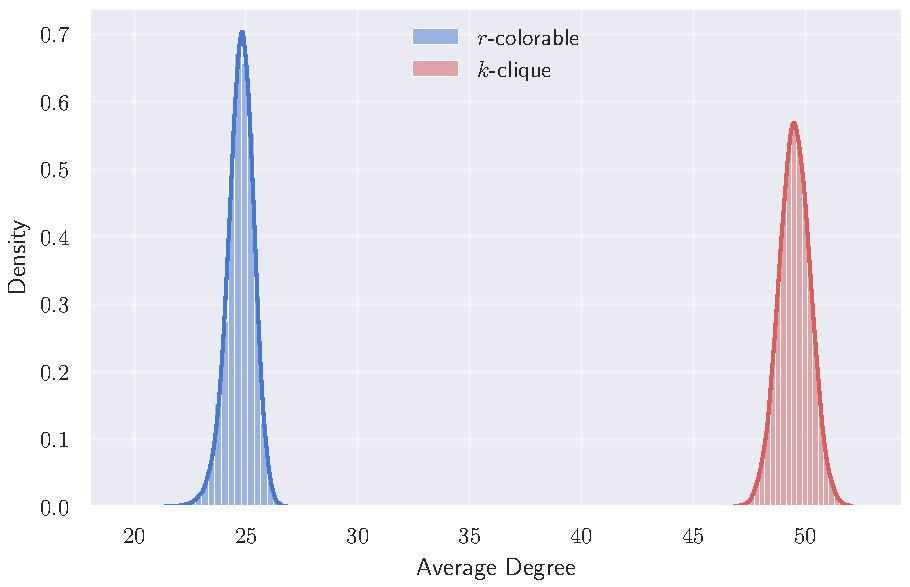
\includegraphics[width=0.9\linewidth]{plots/same-edgeprob.pdf}
    \caption{Histogram with KDE of average degrees for 2-colorable and 3-clique graphs with $N = 100$ and $p = 0.5$}
    \label{fig:avg-degrees}
\end{figure}

\subsection{Hard Cases for Average Degree}
\label{sec:hard-avg-degree}
To avoid the trivial case, we consider the case where the average degree for both graphs is equal. We achieve this by adjusting the edge probability when generating graphs. Starting with the expression for the expected average degree of a $r$-clique graph with $n$ nodes generated using \cref{alg:r-colorable}, we get

\renewcommand{\d}{d_{avg}}


\begin{equation}
\label{eq:r-edgeprob}
    \begin{split}
        \d = p(n-1)\frac{(r-1)}{r}
    \end{split}
\end{equation}
Similarly, for \cref{alg:r-colorable}, we get 
 

\begin{equation}
\label{eq:s-edgeprob}
    \begin{split}
        \d = \frac{s(s-1) + q(n-s) s  +2q (n -s) (n-s-1) }{n}
    \end{split}
\end{equation}
 Here the first term comes from edges within the clique, the second from edges between clique and non-clique nodes and the last from edges between non-clique nodes. Setting \cref{eq:s-edgeprob,eq:r-edgeprob} equal, we can solve for the $q$ where the expected average degree is the same.

\begin{equation}
    \begin{split}
        q = \frac{n  p \left(n - 1 \right)  \frac{r - 1}{r} - s \left(s - 1 \right)}{\left(n - s \right)  \left(n + s - 1 \right)}
    \end{split}
\end{equation}




The adjusted distributions are shown in \cref{fig:same-dist}. While the distribution of r-colorable graphs exhibits a slight left skew and has heavier tails, the high overlap coefficient of 0.9458 indicates that the two distributions are nearly identical. Empirical statistics based on 100,000 graphs with 100 nodes are presented in \cref{tab:same-dist}.


\begin{table}[htbp]
\caption{Empirical statistics based on 100,000 graphs with 100 nodes for the two distributions discussed in \cref{sec:hard-avg-degree}.}
\label{tab:same-dist}
\centering
\begin{tabular}{lrr}
\toprule
  Statistic & $r$-Colorable Graphs & $k$-Clique Graphs \\
\midrule
 Mean & 24.750 & 24.749 \\
 Variance & 0.370 & 0.370 \\
 Skewness & -0.511 & 0.022 \\
 Kurtosis & 1.186 & 0.005 \\
\midrule
  Overlapping Coefficient &\multicolumn{2}{r}{0.9458} \\
\bottomrule
\end{tabular}
\end{table}
% \begin{table}[htbp]
% \caption{Empirical statistics based on 100,000 graphs with 100 nodes for the two distributions discussed in \cref{sec:hard-avg-degree}.}
% \label{tab:same-dist}
% \centering
% \begin{tabular}{llrr}
% \toprule
%   Statistic & $r$-Colorable Graphs & $k$-Clique Graphs \\
% \midrule
%  Mean & 33.000 & 32.997 \\
%  Variance & 0.437 & 0.439 \\
%  Skewness & -0.236 & 0.008 \\
%  Kurtosis & 0.383 & -0.013 \\
% \midrule
%   Overlapping Coefficient (OVL) &\multicolumn{2}{r}{0.971} \\
% \bottomrule
% \end{tabular}
% \end{table}
\todo[color=green]{Include or remove histogram?}

\begin{figure}[htbp]
    \centering
    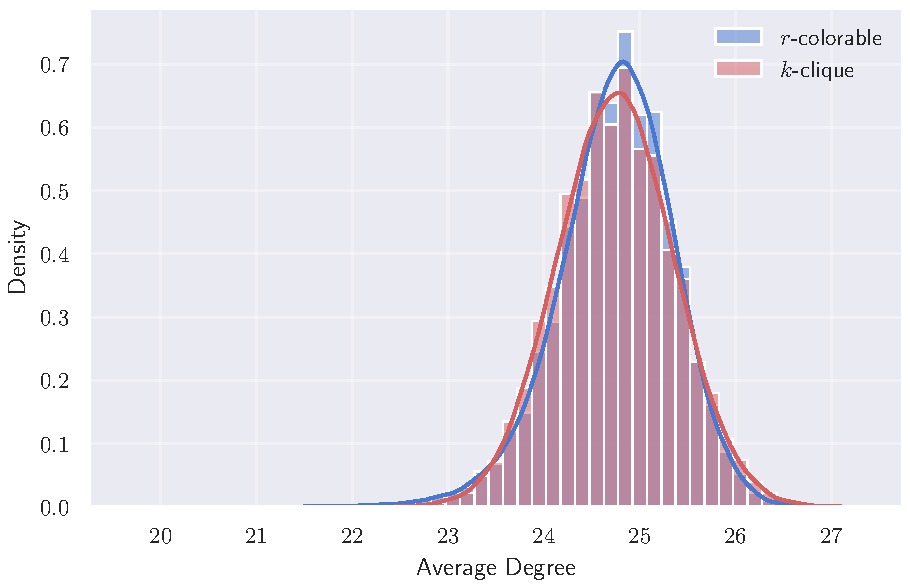
\includegraphics[width=0.9\linewidth]{plots/same-dist.pdf}
    \caption{Histogram with KDE of average degrees for 2-colorable and 3-clique graphs with $N = 100$ and edge probability adjusted to give the same average degree.}
    \label{fig:same-dist}
\end{figure}



\todo[inline]{I think that Vilijar also made some experiments stating that this distribution is easy for more general types of networks. }



\clearpage
\subsection{Architectures (GNNs + Linear Layers)}
\todo{Decide on which models to present and which results to present}
\todo[color=green]{Which r and s to present?}

\begin{figure}[ht]
    \centering
    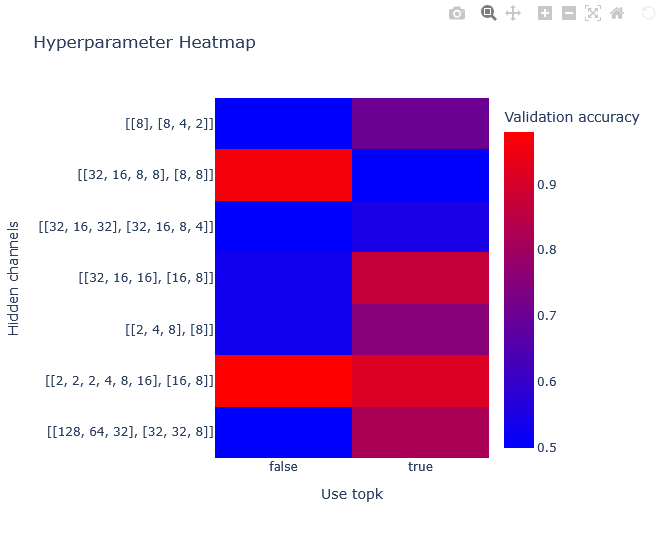
\includegraphics[width=0.8\linewidth]{plots/temp_results.png}
    \caption{Enter Caption}
    \label{fig:enter-label}
\end{figure}

\section{Improvements with the Top $k$ nodes technique}

\todo[inline]{Define pooling, and how it improves the process.}


\section{Connections with Weisfeiler Lehmant}
\begin{itemize}
\item paper about lower bounds for WL algorithm\url{https://people.cs.umass.edu/~immerman/pub/opt.pdf}
\item \url{https://arxiv.org/abs/1810.02244} 
\item Potentially hard case: A pair of graphs $G_1$ and $G_2$ that have the same 
WL-type, but one is $r$-colorable and the other has a $k$ clique. \todo{How to generate this?}
\end{itemize}
